% Haskell is mijn favoriete taal

Het signaalverwerkingsblok maakt een nuttig signaal van de te meten grootheid. Een uitbreiding van dit blok is te zien in \cref{fig:signaalverwerking}.
Van links naar rechts zijn de functies van de blokken als volgt:
\begin{enumerate}
    \item De grootheid, de pH waarde, wordt gemeten. Dit wordt gedaan door de gate-source spanning $U_{GS}$ van de ISFET te meten.
    \item Het signaal wordt gefilterd om de bandbreedte te limiteren.
    \item Er wordt voor de kruisgevoeligheid van de pH sensor gecompenseerd d.m.v. een temperatuursensor.
    \item De waarde van $U_{GS}$ wordt omgerekend naar de pH waarde.
    \item Deze waarde wordt draadloos opgestuurd naar de ontvanger.
\end{enumerate}
Het `enable' blok wordt gebruikt om het signaalverwerkingsonderdeel van het systeem te activeren en te deactiveren. Op deze manier hoeft het systeem alleen maar aan te staan wanneer het nodig is, en wordt er minder energie verbruikt.

% \begin{figure}[!htbp]
%     \centering
%     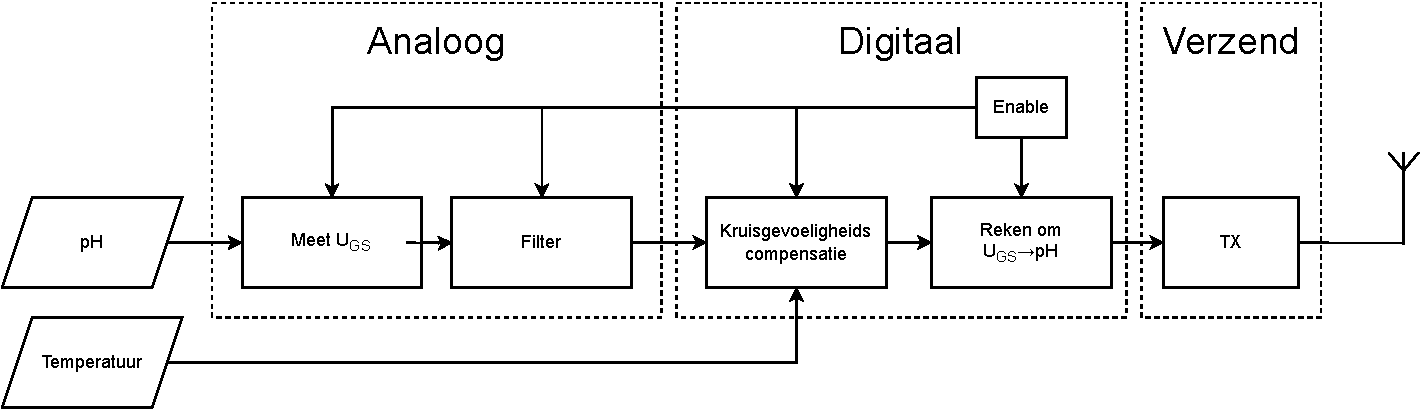
\includegraphics[width=\textwidth]{meetGedeelte.pdf}
%     \caption{Het signaalverwerkende onderdeel van het systeem, onderverdeeld naar het analoge en digitale domein.}
%     \label{fig:signaalverwerking}
% \end{figure}



\begin{figure}[!htbp]
    \centering
    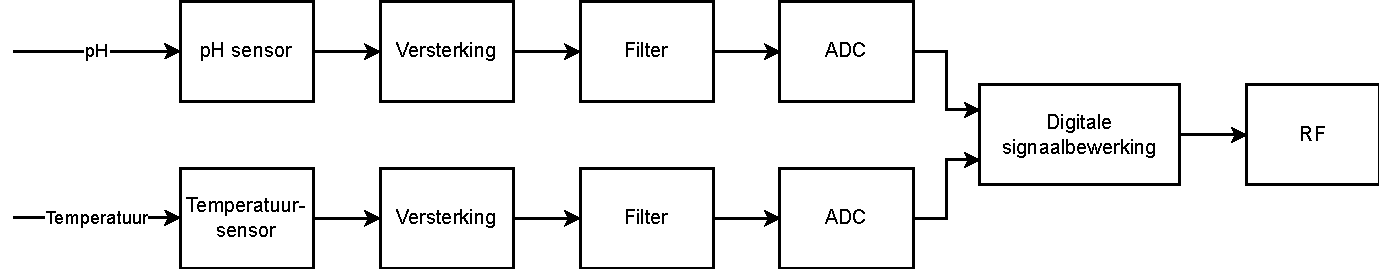
\includegraphics[width=0.95\textwidth]{analogeBewerkingsFunctie}
    \caption{Het analoge gedeelte van de signaalbewerking.}
    \label{fig:analogeBewerkingsFunctie}
\end{figure}


\begin{figure}[!htbp]
    \centering
    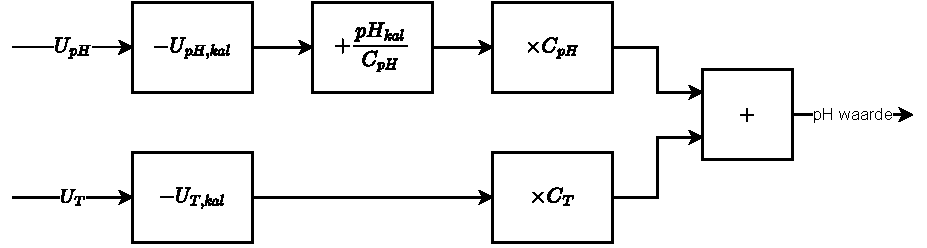
\includegraphics[width=0.95\textwidth]{digitaleBewerkingsFunctie}
    \caption{Het digitale gedeelte van de signaalbewerking.}
    \label{fig:digitaleBewerkingsFunctie}
\end{figure}



% TODO: TAAL
\subsection{Spanningsregeling}
Voor spanningsregeling zijn er meerdere componenten nodig, zoals te zien in \cref{fig:spanningsregeling}. De energy harvesting produceert een spanning, die omgezet moet worden naar iets de rest van het systeem iets mee kan. Deze omgevormde spanning kan dan zowel gebruikt worden voor het opladen van de batterij, als het voeden van de rest van het systeem.
Om de batterij op te laden is een batterijregelingssysteem (BMS) nodig. De BMS kan via een beveiliging de batterij opladen. De beveiliging limiteert de batterijspanning en -stroom. De tweede beveiliging zit tussen de batterij en de rest van het systeem. Deze beveiliging zorgt ervoor dat er niet te veel stroom uit de batterij getrokken wordt, waardoor deze kapot kan gaan. De spanningsregelaar zet de spanning die uit de batterij komt om naar een spanning die gebruikt kan worden door de rest van het systeem.

\begin{figure}[!htbp]
    \centering
    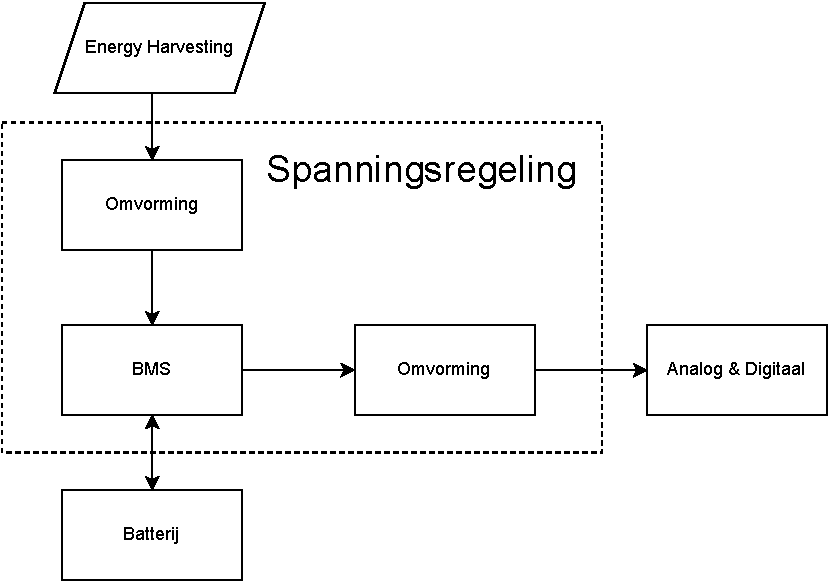
\includegraphics[width=0.7\textwidth]{spanningsRegeling3.drawio.pdf}
    \caption{Het Spanningsregeling van het systeem.}
    \label{fig:spanningsregeling}
\end{figure}

\subsection{TX}
In \cref{fig:functional} is het TX blok het blok dat de data draadloos verstuurt. Dit blok zal direct ingekocht worden; Er zijn namelijk meer dan genoeg kant-en-klare oplossingen beschikbaar om de functie van dit blok te vervullen.


\subsection{Microcontroller}
Een gedeelte van de signaalverwerking zal gebeuren in het digitale domein. Hiervoor is een microcontroller de voor de hand liggende oplossing. Bij het kiezen van een microcontroller moet er een aantal eigenschappen overwogen worden. Een paar van deze eigenschappen zijn:
\begin{itemize}
    \item gebruikte vermogen;
    \item mogelijke slaapstanden;
    \item beschikbare peripherals;
    \item kloksnelheid;
    \item geheugen;
    \item programmeergeheugen;
    \item en de prijs.
\end{itemize}
